\chapter{A New Compton Scanner at the Max Plank Institute for Physics} \label{chap:scanner}

A pulse shape library of interactions in the bulk of a detector can be created by scanning the detector with a collimated gamma source. The position of the collimated source automatically determines two of the three spatial coordinates of an interaction vertex. However, additional information is required to determine the third. The Compton effect can be exploited for this purpose~\cite{Petry1993,Vetter2000,Abt2008,Dimmock2009,Ha2013,vonSturm2017}. A common approach is to select gammas which scatter at right angles with respect to the source beam-axis with a horizontal slit collimator. The slit position automatically determines the coordinate in question~\cite{Vetter2000,Dimmock2009,Ha2013,vonSturm2017}. At least one auxiliary detector is needed to capture the scattered gammas. While effective, this approach requires a vertical scan with the slit collimator for each position of the source. This results in prohibitively long measurement times when dealing with large detectors. Another approach involves comparing pulse shapes from vertical and horizontal collimated source scans in highly segmented detectors~\cite{Crespi2008,DeCanditiis2020}.

A novel Compton Scanner was built at the Max Planck Institute for Physics in Munich which drastically reduces the measurement time necessary to create a pulse shape library with known interaction vertices~\cite{compton_scanner}. A position-and-energy sensitive detector or ``camera'' is implemented to capture the scattered gammas from the detector under study, which eliminates the need for horizontal slit collimators. Scatters are no longer restricted to 90$^{\circ}$, but rather a wide-range of angles are accepted, only restricted by the angular coverage of the camera.

\section{Working Principle}\label{sec:workingprinciple}

The detector under study is irradiated vertically with a gamma beam to induce pulses along the beam axis. The use of a collimated gamma source with a known position automatically determines the $x$ and $y$ coordinates of the induced pulses. The Cartesian coordinate system used throughout the text is presented in Fig.~\ref{fig:workingprinciple}, with the gamma beamed aligned with the $z$-axis. 

\begin{figure}[!tbh]
    \centering
    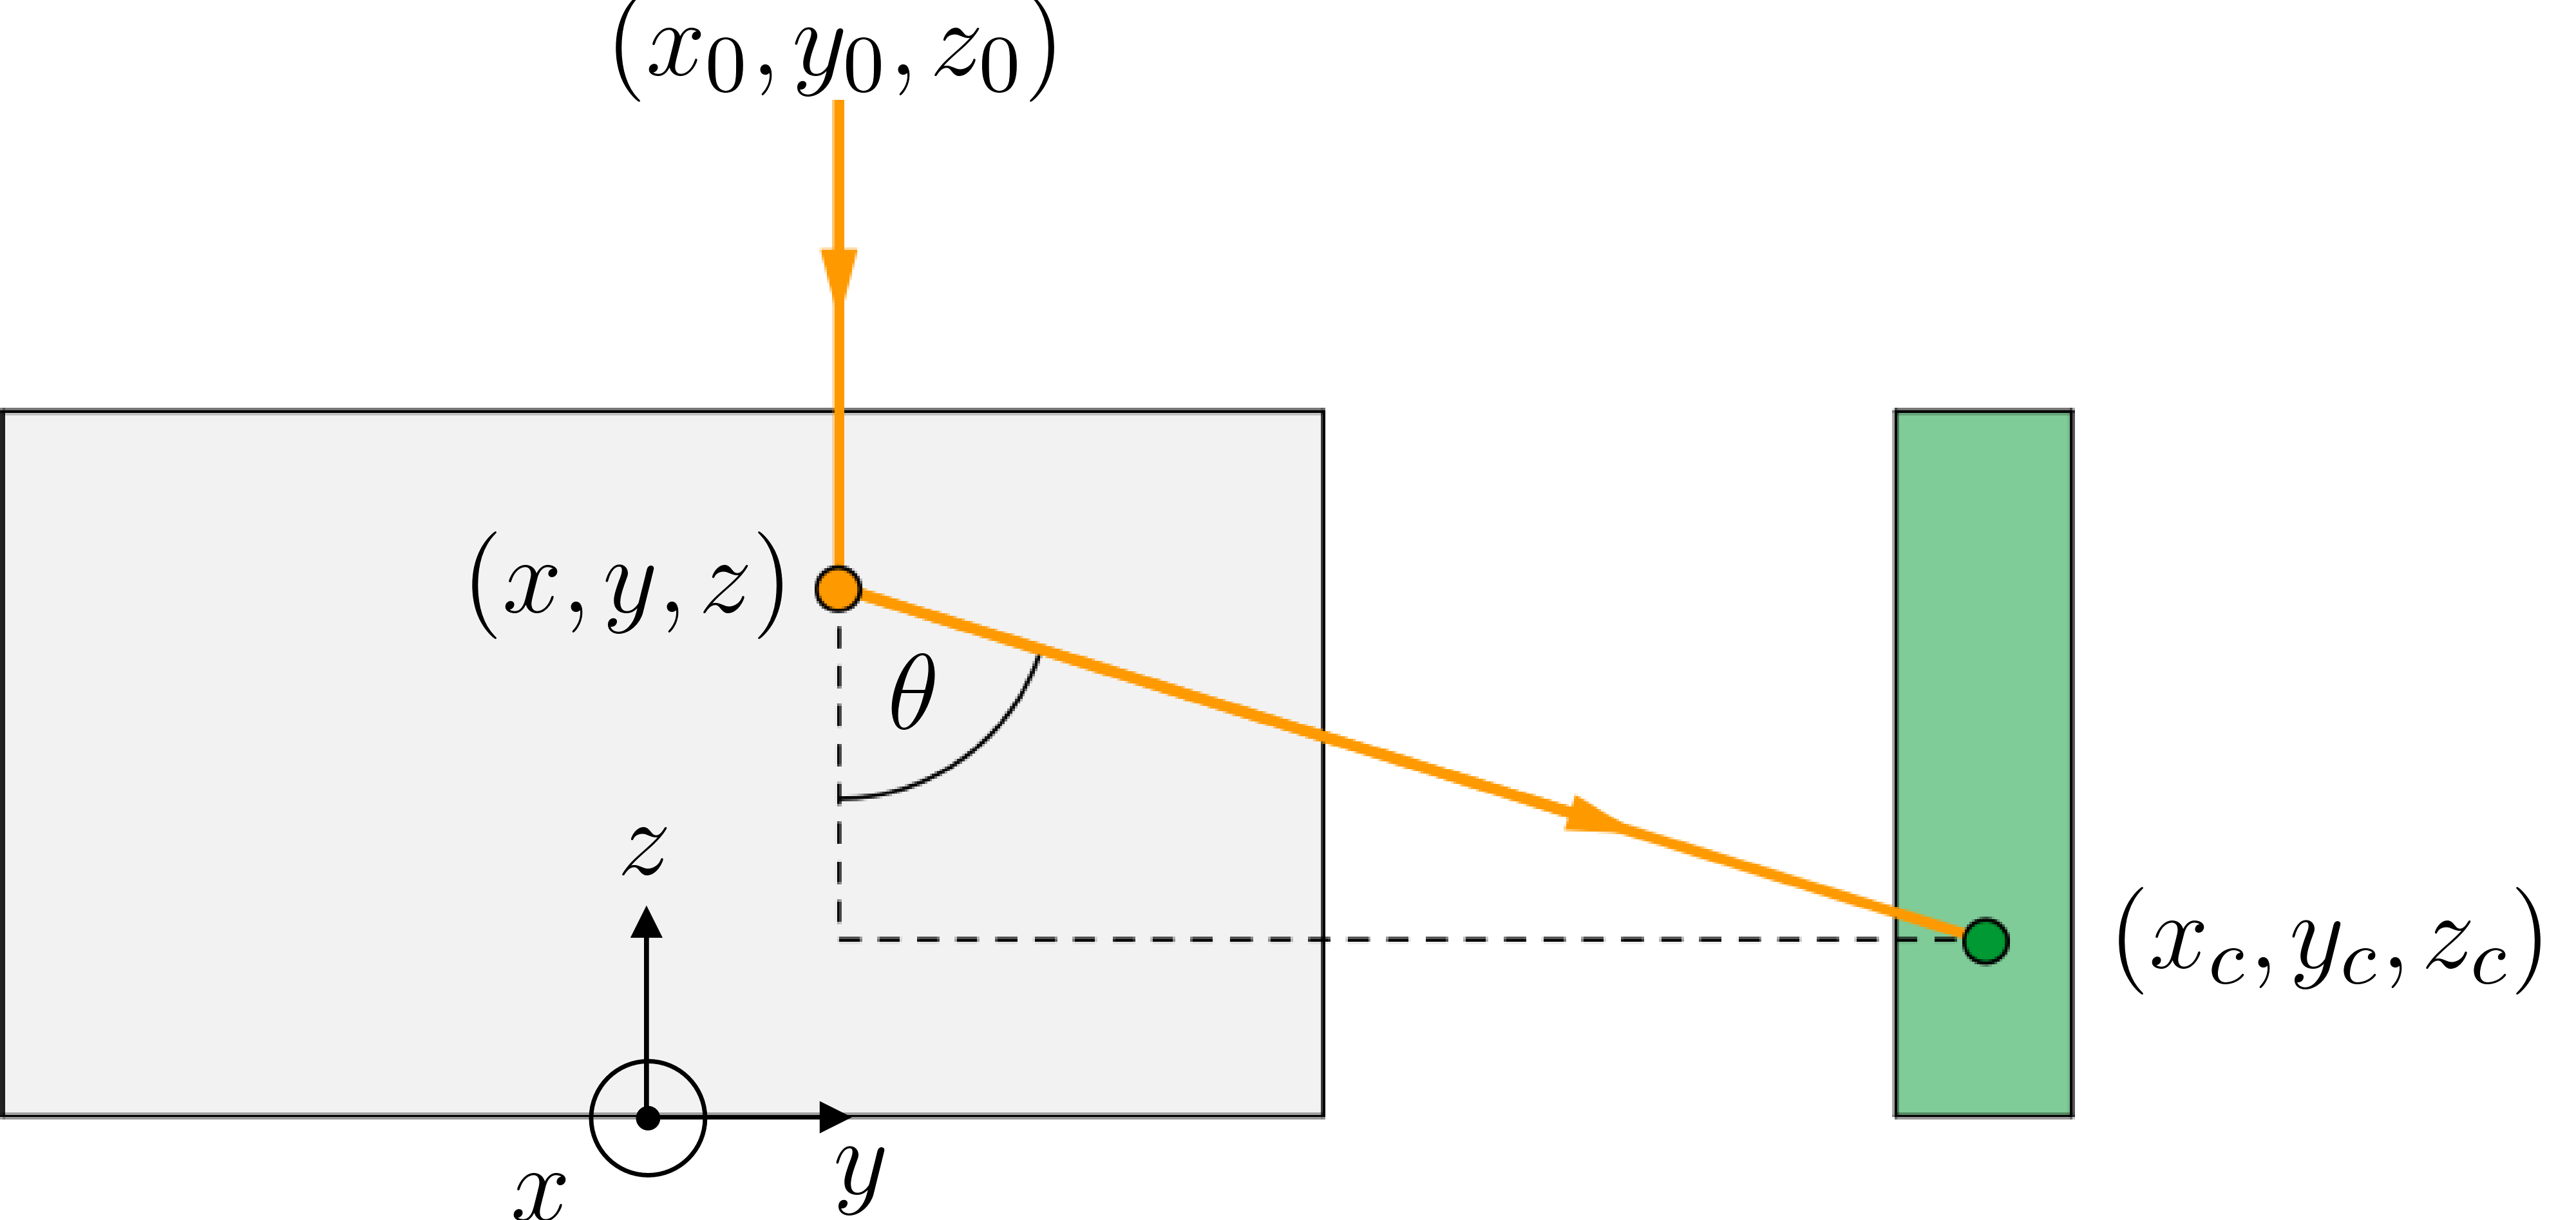
\includegraphics[width=4in]{figs/scanner/WorkingPrinciple_labeled_width_4in.png}
    \caption{An example gamma trajectory (orange) in a single-site detector event. The detector (illustrated as a gray rectangle) is irradiated from the top by a collimated source located at $(x_0, y_0, z_0)$, resulting in a beam axis parallel to the $z$-axis. The gamma scatters at $(x,y,z)$ and is fully absorbed in the camera (green rectangle) at $(x_c, y_c, z_c)$. The camera, source and detector are in a common system of coordinates, whose origin is at the center bottom of the detector~\cite{compton_scanner}.}
    \label{fig:workingprinciple}
\end{figure}

The incoming gammas Compton scatter with an energy dependent probability, deflecting from the beam axis. The resulting Compton angle, $\theta$, is determined using the relationship between the incoming gamma energy, $E_\text{in}$ and the energy deposited in the detector, $E_\text{det}$, via the well known Compton scattering formula~\cite{compton}   

\begin{equation} \label{eq:compton}
    \cos(\theta) = 1 - \dfrac{m_ec^2 E_\text{det}}{E_\text{in} \left(E_\text{in} - E_\text{det}\right)}~.
\end{equation}

While most Compton scattered gammas are fully absorbed within the detector or passive materials in the surrounding structure, some are fully absorbed within the camera. The relationship between emitted and camera-absorbed scatters is determined by the $E_\text{in}$ and the angular coverage, position, thickness and material of the camera. If a gamma is fully absorbed by the camera, the location of the scattering vertex in the detector, $(x,y,z)$, is reconstructed with a simple trigonometric calculation,
\begin{equation} \label{eq:ztheta}
    z = z_\theta \equiv z_c + \sqrt{(x_c-x_0)^2 + (y_c-y_0)^2} \;\cot(\theta)~. 
\end{equation}
The value of $z$ obtained from this calculation is referred as $z_\theta$ throughout the text. Events which scatter in the detector and are fully absorbed in the camera are selected by cutting on events coincident in the detector and camera whose combined energy equal $E_\text{in}$. In addition, this population also contains events which multiple scatter in the detector, camera, or both. Multiple scatters in the detector produce an incorrect result when using Eq.~\ref{eq:ztheta} as exemplified by Fig.~\ref{fig:cone_validation}. 
\begin{figure}[!tbh]
    \centering
    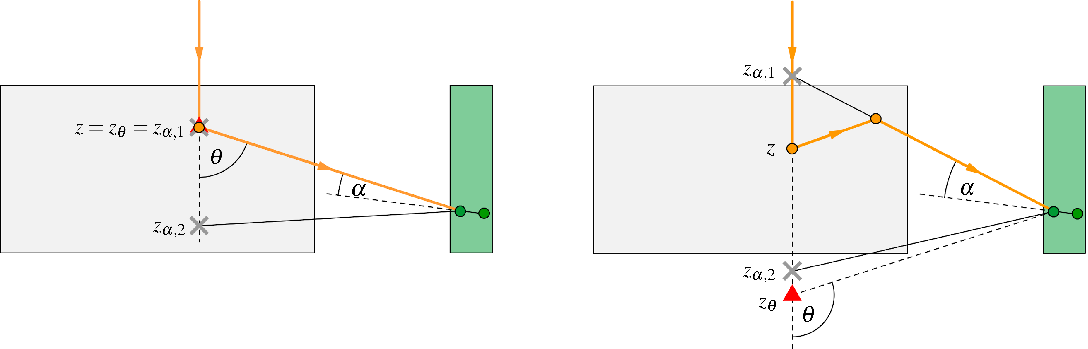
\includegraphics[width=6in]{figs/scanner/alpha_theta.pdf}
    \caption{An example gamma trajectory in a single(multi)-site detector event is depicted on the left(right). In the single-site event, one of the $\alpha$-reconstructed $z$-positions (marked with a gray cross) coincides with the value produced by the $\theta$-reconstruction (marked with a red triangle). The true scattering vertex (marked with an orange dot) is thus found. In the multi-site event, neither $\alpha$-reconstructed $z$ position coincides with the value produced by the $\theta$-reconstruction. Therefore, the algorithm fails to reconstruct the position of the scattering vertex~\cite{compton_scanner}.}
    \label{fig:cone_validation}
\end{figure}
However, multiple scatters in the camera are up to a degree desirable since they provide a detector-independent way of reconstructing the position of the scattering vertex. Therefore, events with two hits in the camera are chosen as optimal for position reconstruction. Due to the limited timing resolution of the camera, the order of camera hits -- which is needed for the detector-independent reconstruction -- is unknown. Each possible ordering of hits results in up to two possible reconstructed $z$ values, $z_{\alpha,1}$ and $z_{\alpha,2}$. To determine these values, the angle $\alpha$ depicted in Fig.~\ref{fig:cone_validation} is determined via the Compton scattering formula but this time with the first and second hit energies, $E_\text{cam}^i$ and $E_\text{cam}^f$, 
\begin{equation} \label{eq:compton_alpha}
    \cos(\alpha) = 1 - \dfrac{m_ec^2 E_\text{cam}^i}{(E_\text{in} - E_\text{det}) \left(E_\text{in} - E_\text{det} - E_\text{cam}^i\right)} = 1 - \dfrac{m_ec^2 E_\text{cam}^i}{(E_\text{cam}^i + E_\text{cam}^f) \left(E_\text{cam}^f\right)}~.
\end{equation}
In the scenarios depicted in Fig.~\ref{fig:cone_validation}, a virtual cone is back-projected and intersects the beam axis at $z_{\alpha,1}$ and $z_{\alpha,2}$. This method is referred throughout the text as the $\alpha$-reconstruction, whereas employing Eq.~\ref{eq:ztheta} is referred to as the $\theta$-reconstruction. If one of these values matches the $z_\theta$ calculated from Eq.~\ref{eq:ztheta} (using the coordinates of the first camera hit for $(x_c, y_c, z_c)$) the reconstruction is considered to be validated. If neither coincides, then the order of the hits is reversed and the process is repeated. If no matches are found in either permutation the event fails reconstruction and is categorized as a candidate detector multi-site event. The process can be extended to any camera $n$-multiplicity event; nevertheless, such events are increasingly rare and the number of scenarios to be analyzed grows as $n!$.

A pulse shape library of the detector under study is generated by moving the collimated source to different ($x_0$, $y_0$)-positions and reconstructing (with or without validation) the various scattering vertices that form along the beam axis in the detector. Note that to obtain a similar result with a horizontal slit collimator, the slit has to scan the detector vertically for each ($x_0$, $y_0$)-position.

\section{Requirements} \label{sec:requirements}

To ensure a detected event is indeed a Compton scattered gamma, its full energy must be contained in the detector under test and the camera. This energy must be known; therefore, a monoenergetic gamma source is required. Additionally, the energy of the monoenergetic gammas should be high enough to penetrate through the entire bulk of the detector while having a high probability of Compton scattering. An activity several hundred MBq is necessary but not sufficient to keep the measurement time for each position of the source under a day. The additional requirements of the Compton scanning system follow.

A substantial decrease in measurement times is obtained with the implementation of the camera compared to a horizontal slit collimator. The camera must be compact to fit in a modular frame and easily moved to target different regions of the detector under study. Additionally, its active volume thickness and density should be sufficient to fully absorb gammas at the scattered energies. The frame should be mobile and able to fit around any in-cryostat Ge detector, allowing for its study without removal from its vendor cryostat. 

The target spatial resolution of the Compton Scanner should be less than $\pm1\,\text{mm}$ in all dimensions. This value is compatible with the volume of 2\,MeV charge clouds expected from \novbb{} interactions~\cite{Abt2007}. To achieve the desired spatial resolution in the $x$ and $y$ dimensions the diameter of the collimated beam should not exceed 2\,mm throughout the detector volume. Gamma collimation of the desired energies requires several centimeters of high-density material~\cite{Thoraeus1965} such as lead or tungsten. Finally, obtaining a $\pm1\,\text{mm}$ resolution in z, will ultimately depend on the spatial and energy resolution of the camera and its proximity to the detector. 

To accurately reconstruct the position of the scattering vertex using Eq.~\ref{eq:ztheta}, the position of the detector and the main components of the Compton frame -- the source and the camera -- must be known and aligned in a common system of coordinates. This last requirement can be fulfilled with the instrumentation already in place, systematically scanning the detector and camera with the source and fitting the resulting detector event rate.

\section{Components} \label{sec:components}

A common frame houses the main components of the Compton scanner as shown in Fig.~\ref{fig:comptonscanner}. The frame consists of four vertical MayTec\textsuperscript{\tiny\textregistered}~\cite{maytec} aluminum beams mounted on an annular base which are stabilized by additional beams at the top of the frame forming a cross. A separate crossarm (shown in Fig.~\ref{fig:full_setup}) guides cables exiting the frame at the cross and houses a motor controller. 
\begin{figure*}[tbh]
    \centering
    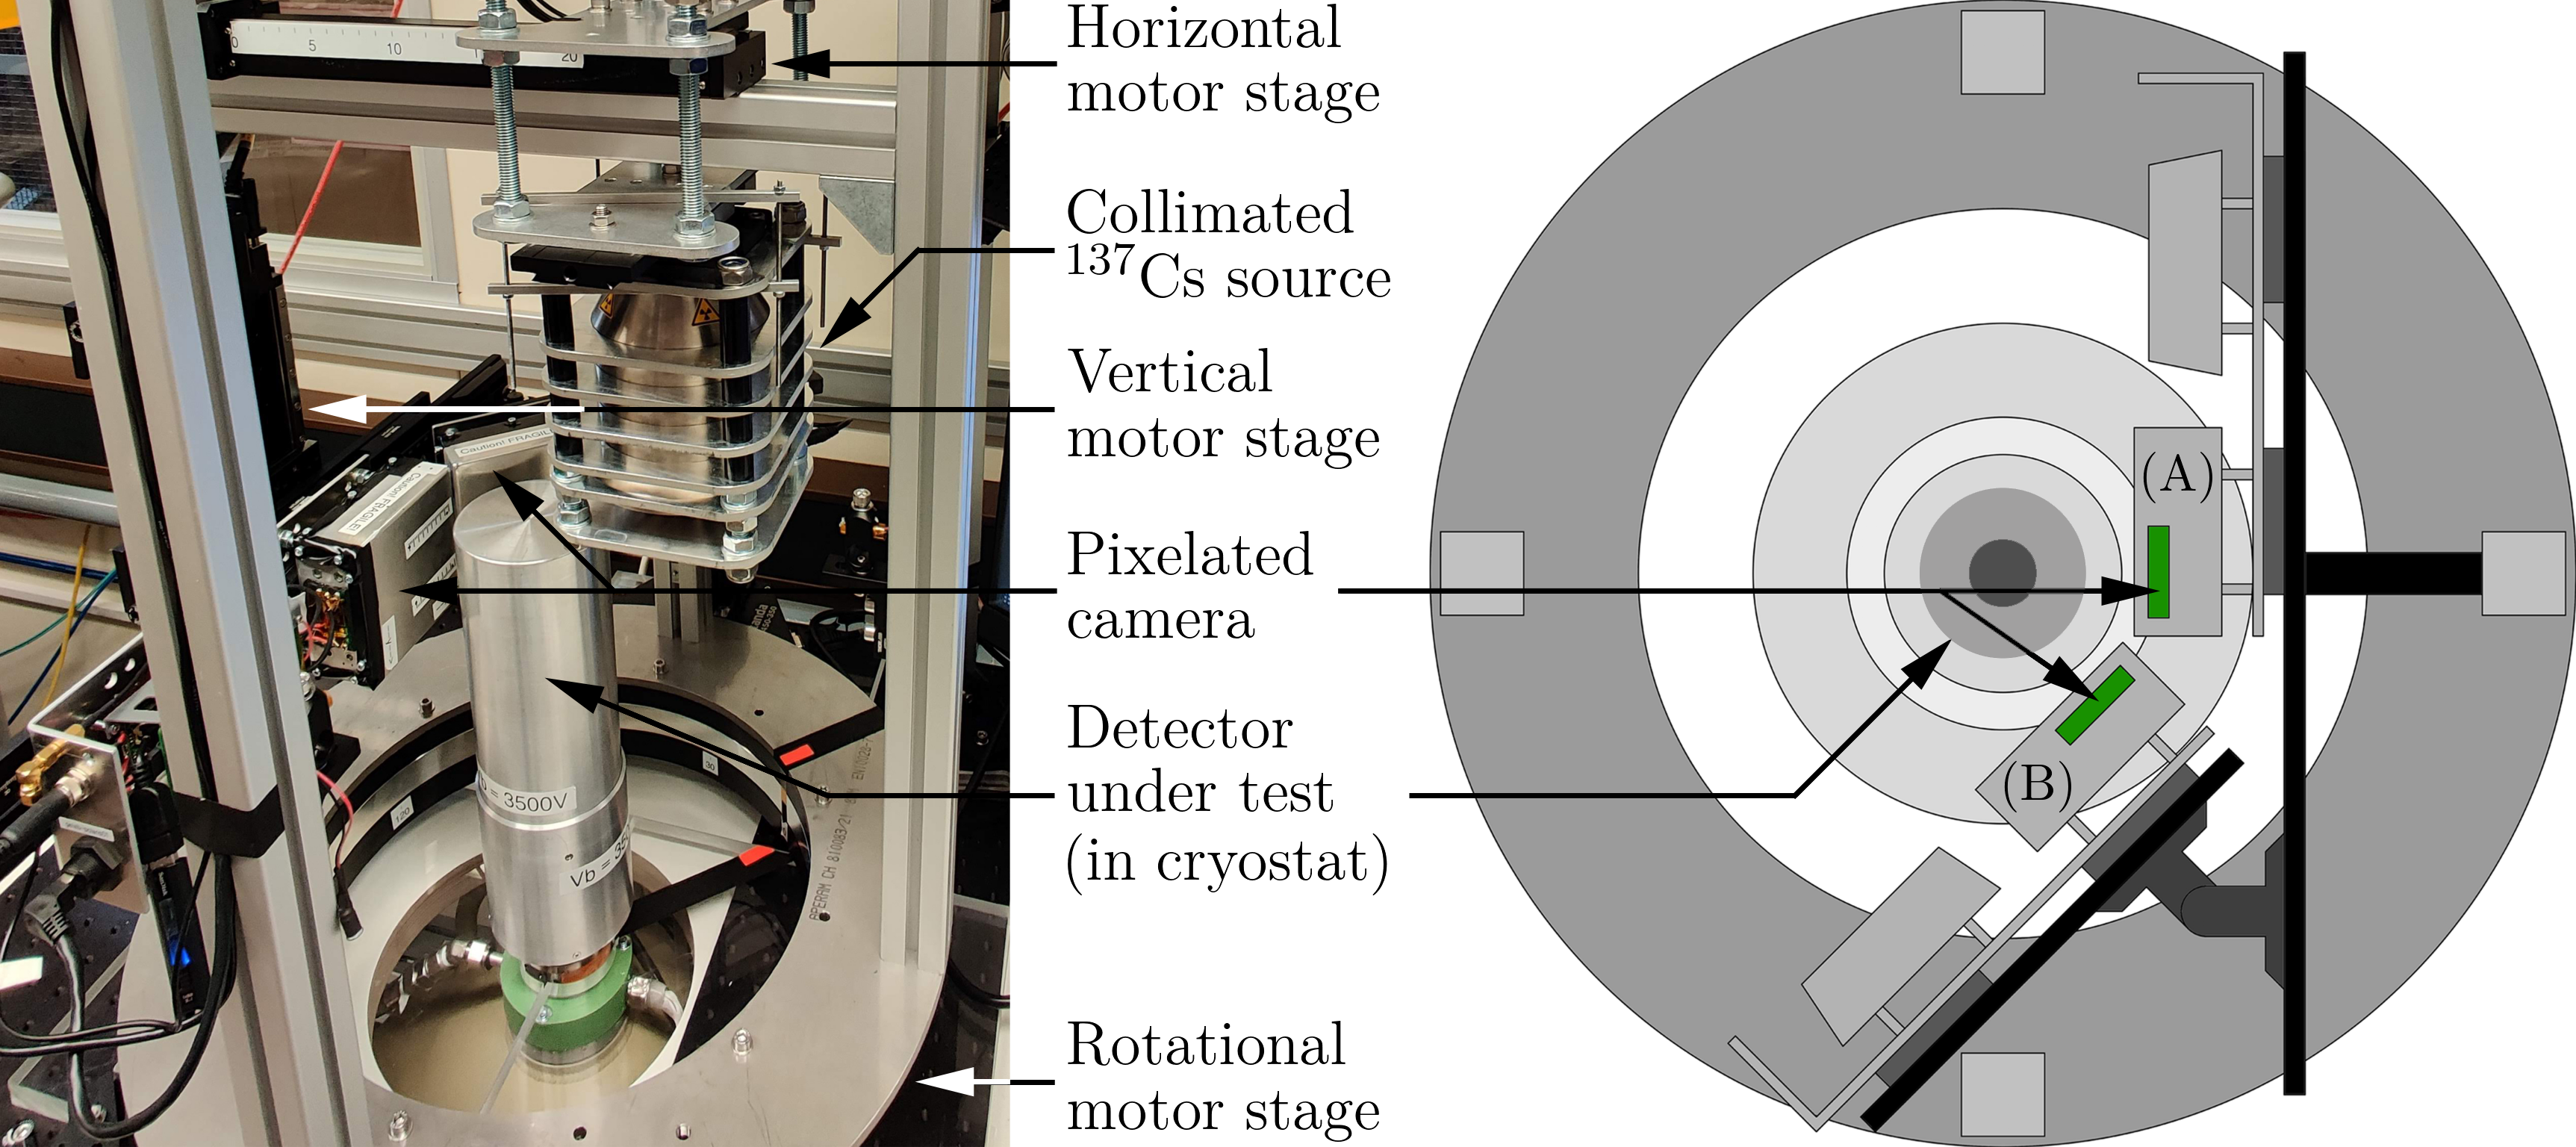
\includegraphics[width=6in]{figs/scanner/ComptonScannerSetup_updated_labeled_width_6_9in.png}
    \caption{The main components of the Compton scanner, including two camera modules (A,B), are pictured on the left. A top view schematic showing the position of the cameras relative to a centered detector (in cryostat) is depicted on the right.}
    \label{fig:comptonscanner}
\end{figure*}

The vertical and horizontal translational motor stages (STANDA\textsuperscript{\tiny\textregistered} 8MT50-200BS1-MEn1~\cite{standa}) are mounted on one of the columns and on an additional horizontal aluminum profile respectively. They can be operated with a precision of 5\,$\upmu$m while under heavy loads. The camera and source are mounted on the vertical and horizontal motor stages respectively. The annular base sits on the rotational motor stage (STANDA\textsuperscript{\tiny\textregistered} 8MRB450-360-60-MEn2) which has a precision of 0.15\textdegree. 

The diameter of the opening of the annular base, combined with the use of a low-profile camera, allows the frame to be mounted around cryostats with diameters of up to 130\,mm. To center the cryostat within the Compton frame, two line lasers mounted on the vertical aluminum profiles are used. The frame and rotational motor stage are fixed along a $600\,\text{mm} \times 600\,\text{mm}$ aluminum breadboard, with a $300\,\text{mm} \times 300\,\text{mm}$ cutout.

\subsection{\CsS{} Source}

The Compton effect dominates in the 200-8000\,keV range as shown in Fig.~\ref{fig:attenuation}. With an energy of \Cs\,keV~\cite{Firestone}, the monoenergetic gamma peak of \CsS{} is in the ideal range where the Compton to Photoelectric effect ratio is favorable, allowing for a mean free path of around 26.9\,mm in Ge~\cite{NIST}. Once the gammas scatter within the detector, their energy should be sufficient to escape and be absorbed in the camera. For scattering tracks perpendicular to the incoming gamma trajectory, 373\,keV is deposited in the Ge. The scattered 289\,keV gammas have a mean free path of 16.8\,mm~\cite{NIST} and can thus have sufficient probability to escape the detector. While higher energies would provide higher penetration depths, both for the incoming and scattered gammas, gammas with these energies become increasingly hard to collimate, and higher energy scatters would not favor absorption in the camera. 

As stated in Section~\ref{sec:requirements}, a source of several hundred MBq is needed, therefore a 740\,MBq \CsS{} source was chosen. The source is cylindrical and has an active diameter of 0.9\,mm. To create the narrow beam required to irradiate the detector, the source is embedded in the collimator depicted in Fig.~\ref{fig:sourcecollimator}.

\begin{figure}[tbph]
	\centering
	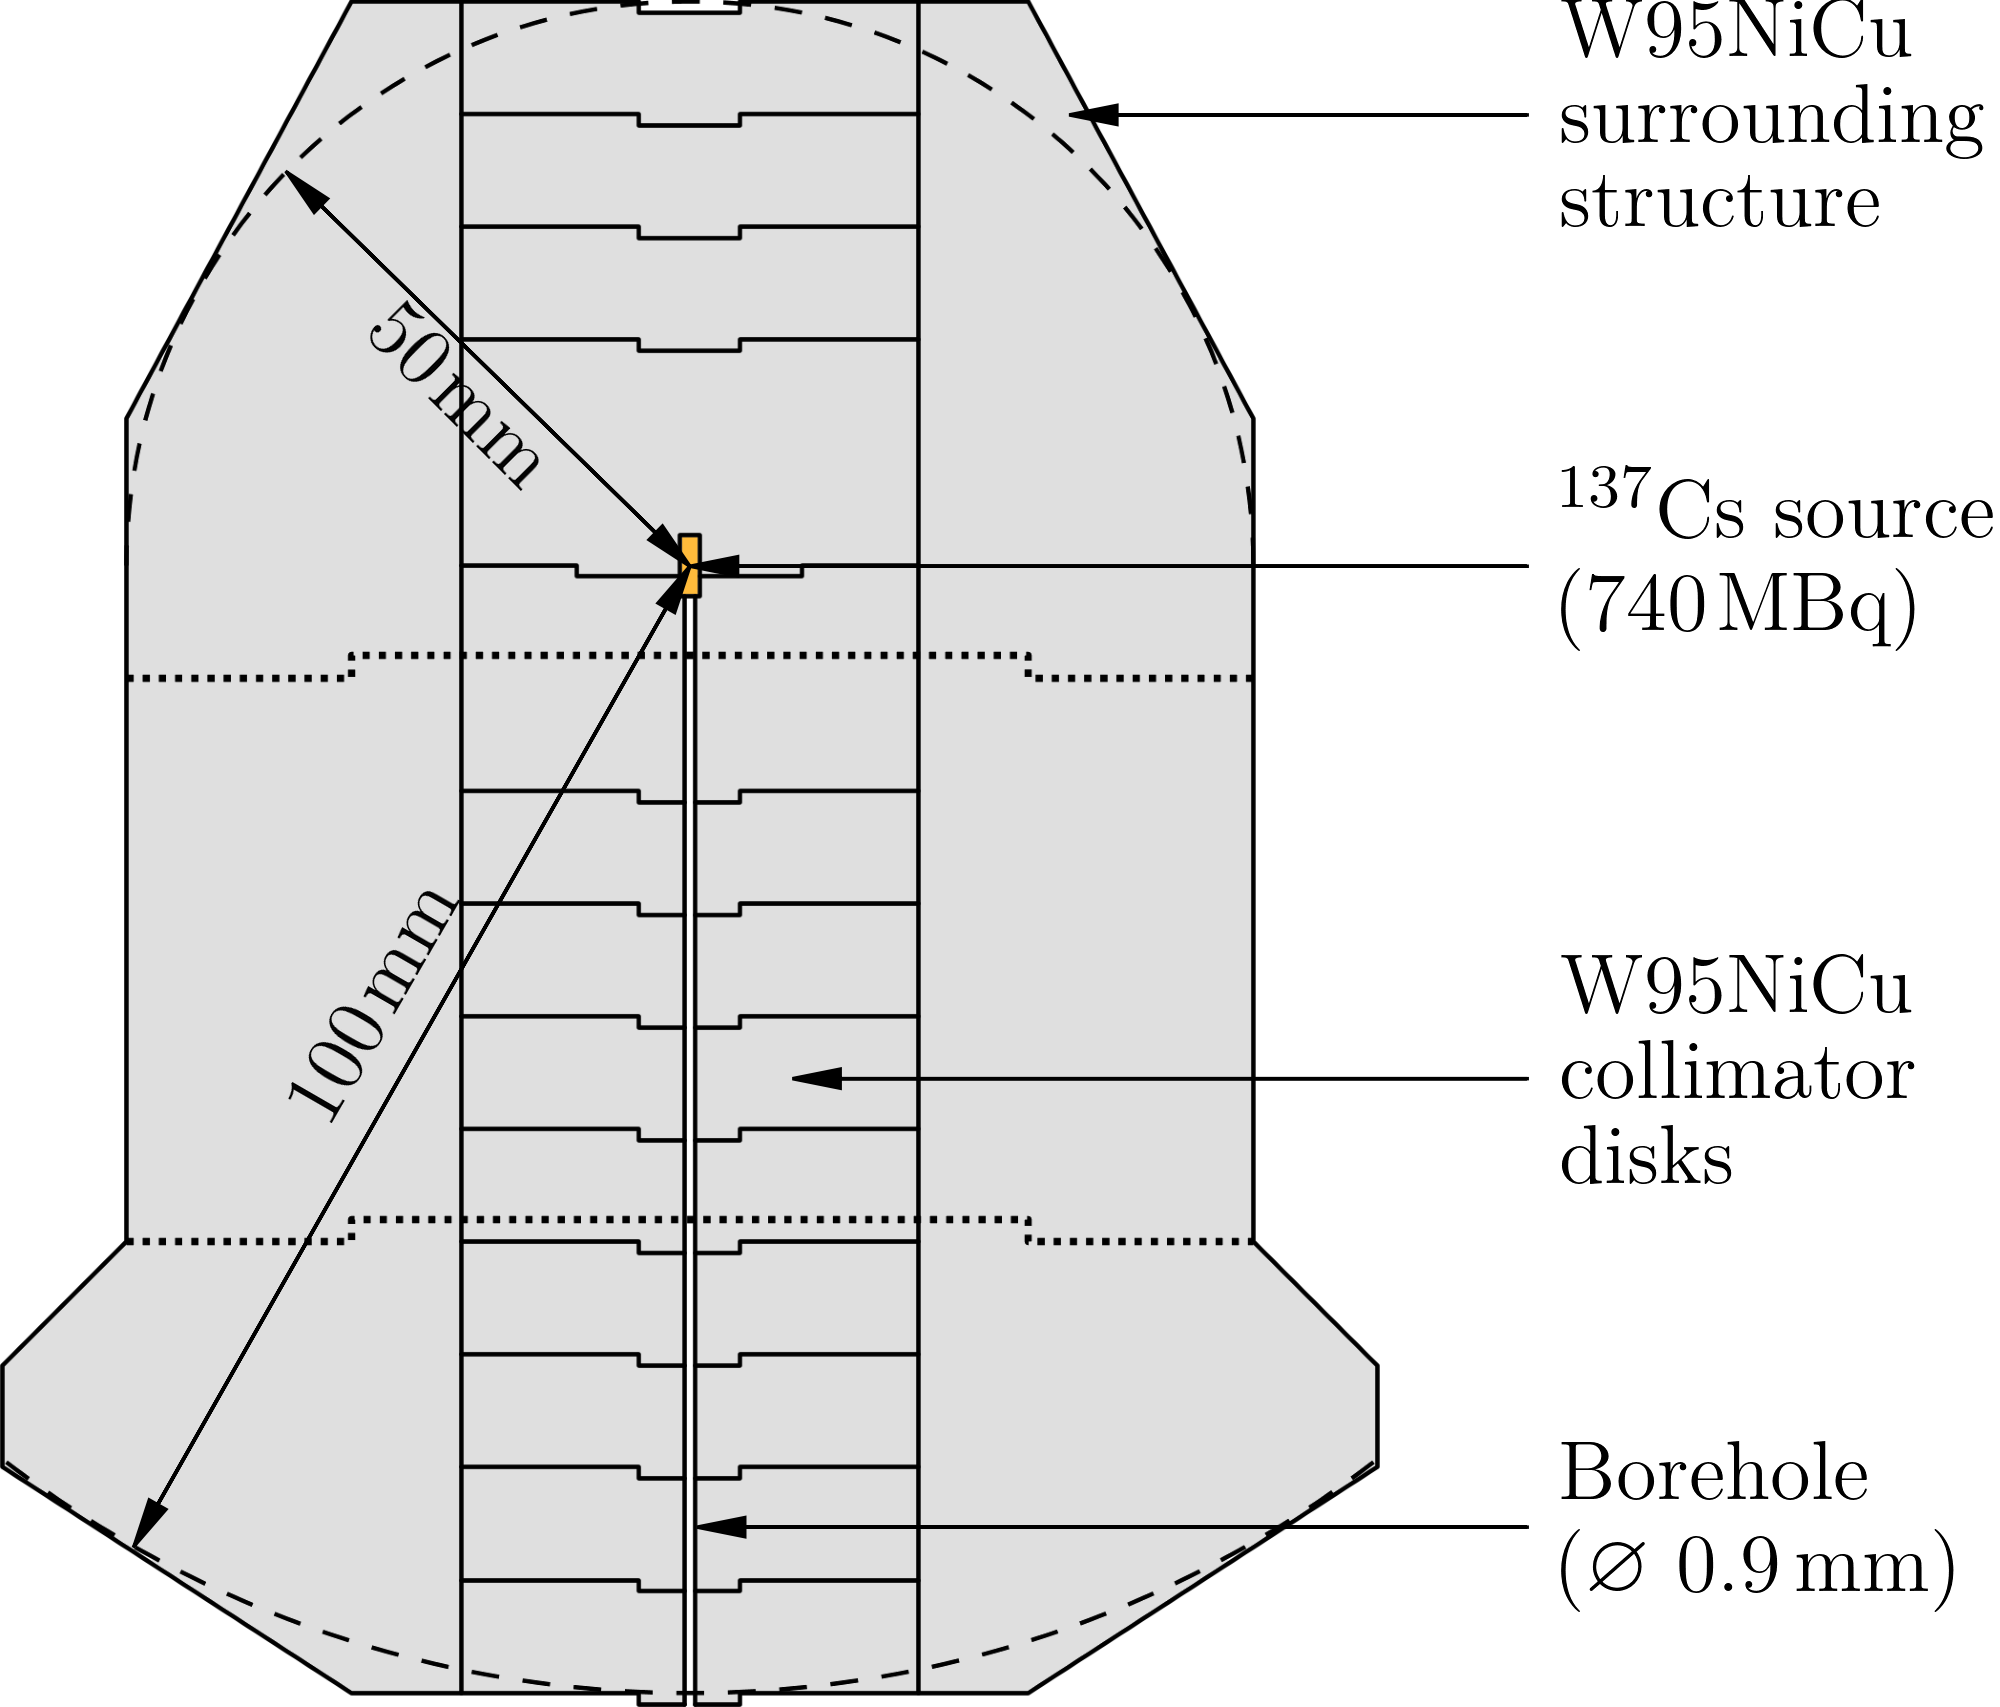
\includegraphics{figs/scanner/ComptonScanner_SourceCollimator_updated_labeled_width_4in.png}
	\caption{Schematic cross-section of the apparatus used to collimate the \CsS{} source~\cite{compton_scanner}.}
	\label{fig:sourcecollimator}
\end{figure}

The collimator was fabricated in its entirety with the tungsten alloy, W95NiCu. The source is embedded in the top of nine concentric annuli which are stacked to form a 100\,mm long borehole which permits vertically emitted gammas to escape the collimator without obstruction. Additional material is placed around the disks such that there is 100\,mm of tungsten alloy between the source and detector for any downward, but not vertically emitted gammas. The diameter and length of the borehole results in a collimated beam with an aperture angle of~0.26\textdegree. This results in a 2.2\,mm beam spot 140\,mm away from the collimator opening. Most in-cryostat detectors fit within this range. Downward gamma rates are attenuated by a factor greater than~$10^{7}$ outside the beam cone. 

Four additional disks are placed on top of the source, along with additional surrounding material to provide at least 50\,mm of tungsten alloy between the source and the personnel handling the source. 

\subsection{Camera System}\label{subsec:camera}

The camera should be capable of fully absorbing the 289\,keV perpendicularly scattered gammas in its active volume while providing good energy and position resolutions. The natural choice of detector that meets these requirements is a pixelated CZT detector. Unlike pixelated silicon detectors, which are limited to a thickness under a couple millimeters~\cite{Si_thickness}, a depletion region thickness of the order of~10\,mm can be obtained in CZT. Note that the mean free path of 289\,keV gammas in CZT is around 11.2\,mm~\cite{NIST}. 

The camera consists of two customized OEM modules produced by H3D, Inc.~\cite{H3D}, also referred to as camera (A) and camera (B) throughout the text. Within the aluminum enclosure of each module four pixelated $22\times22\times10\,\text{mm}^3$ CZT crystals are mounted with a 2\,mm separation between them. The cathode is oriented such that it covers the whole $22\times22\,\text{mm}^2$ surface facing the germanium detector. A segmented anode covering the same area with $11\times11$ pixels is located 10\,mm opposite to the cathode. The arrangement of the CZT crystals within a camera module and the pixel structure is shown in Fig.~\ref{fig:camera}.
\begin{figure}[!tbh]
	\centering
	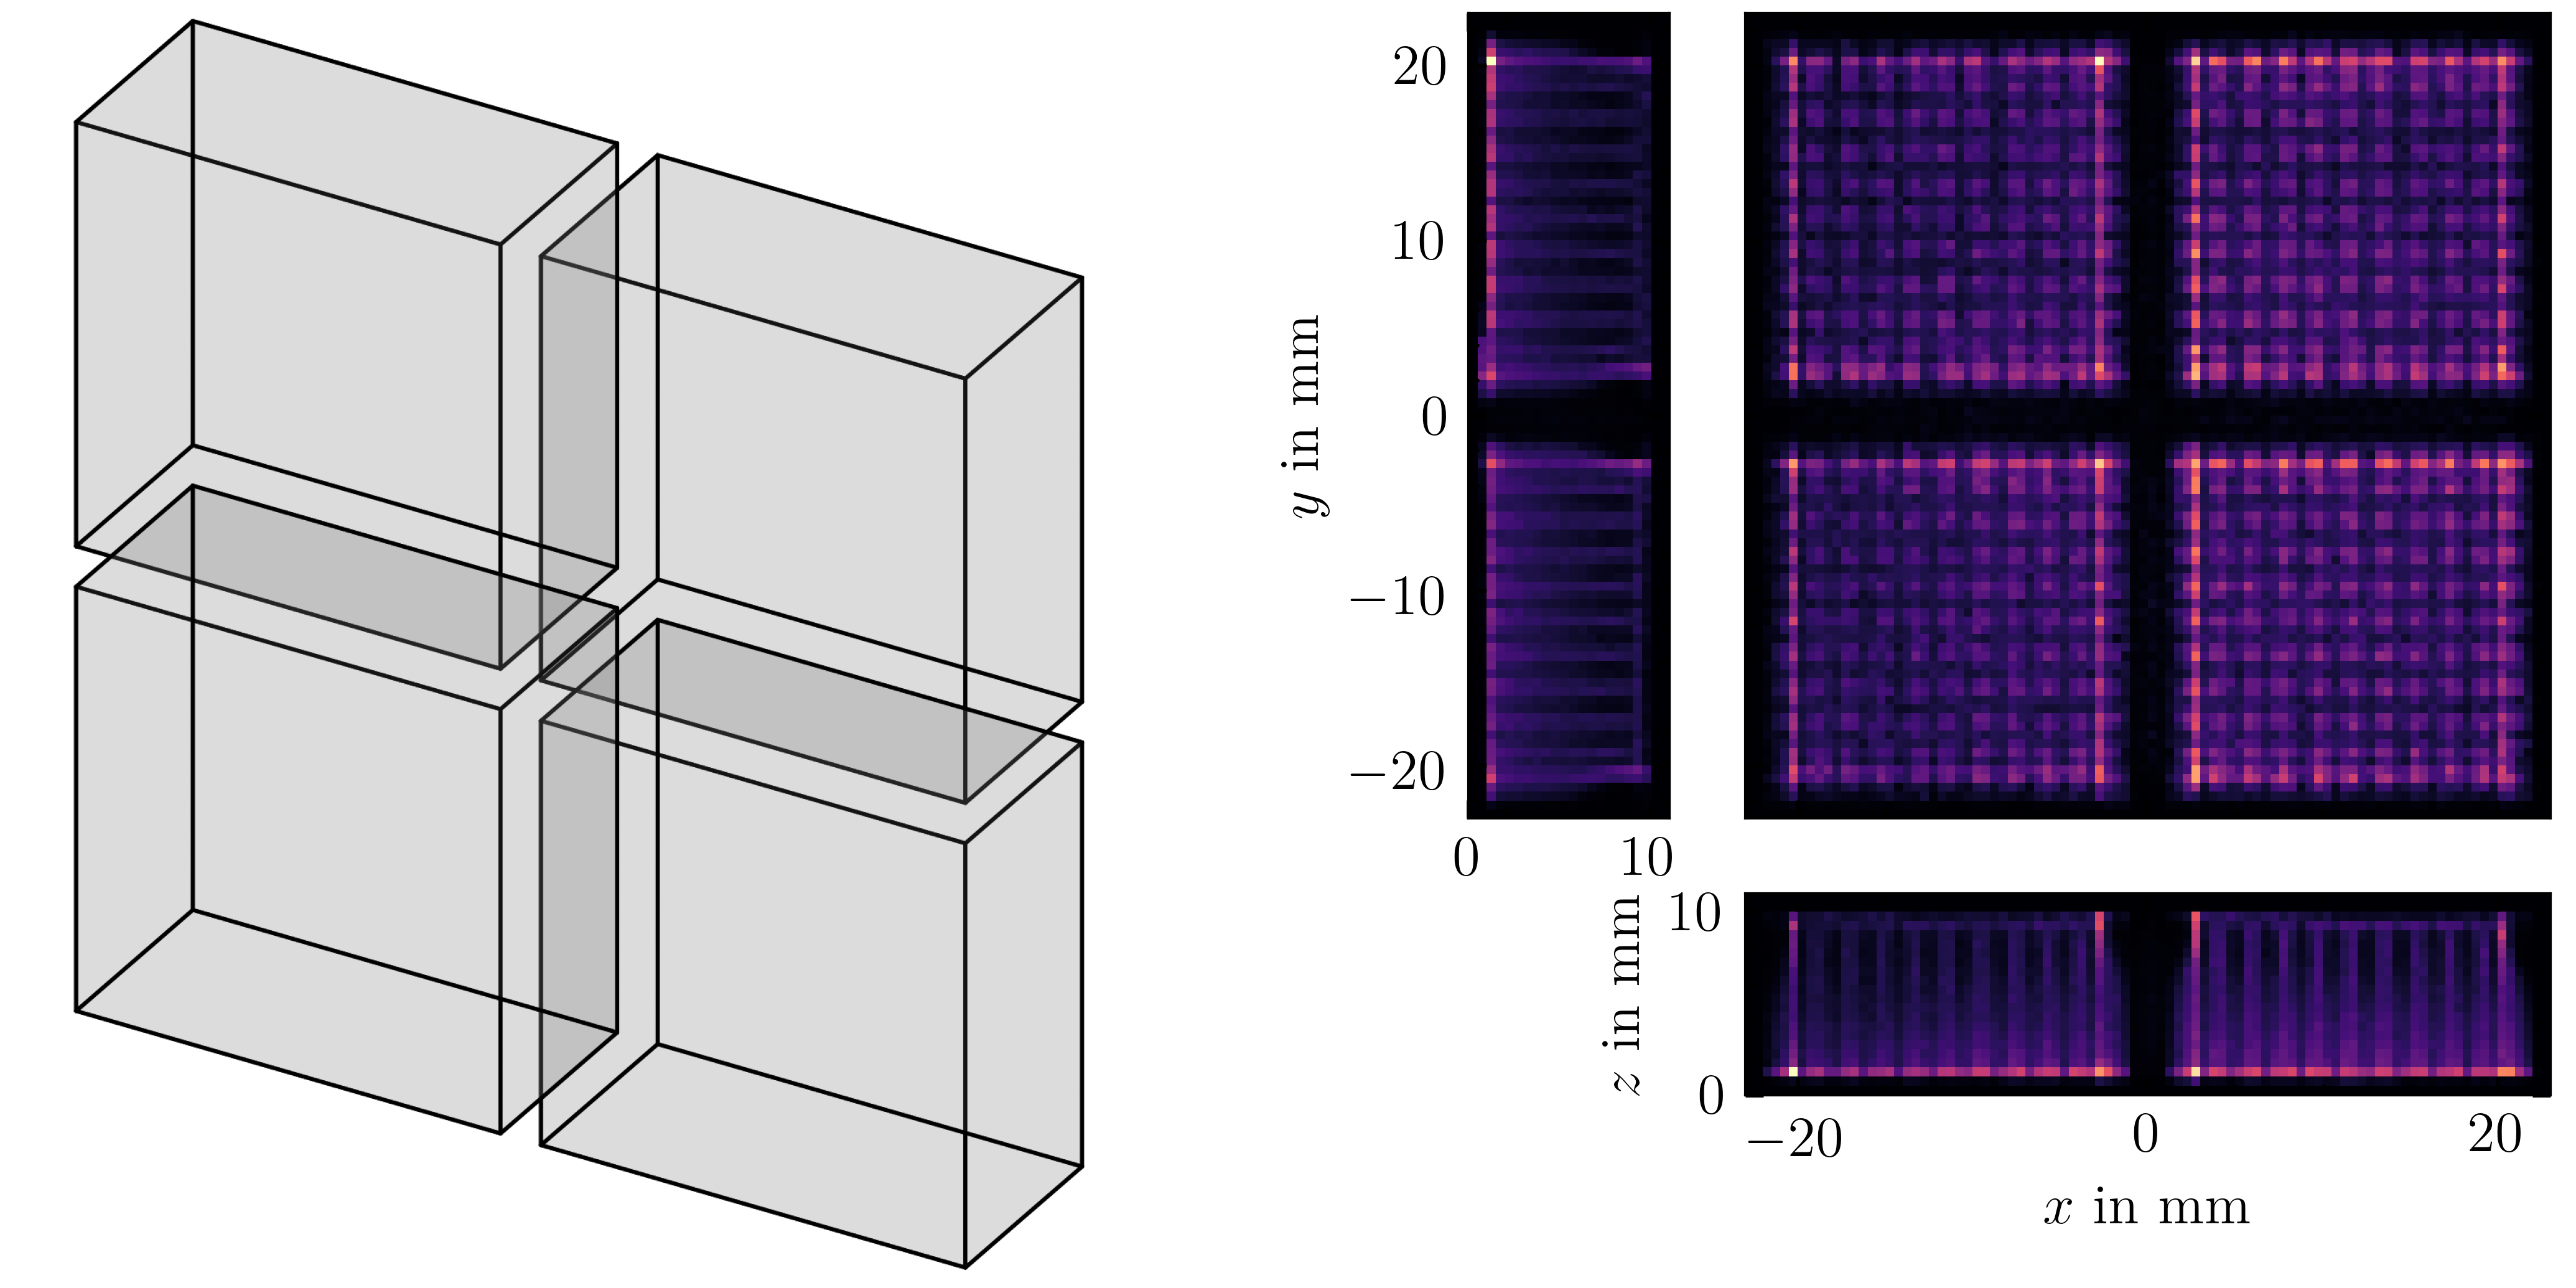
\includegraphics[width=6in]{figs/scanner/caemra.png}
	\caption{A representation of CZT crystal arrangement within the camera module is shown on the left. This geometry is reflected in the event position data shown on the right. For this example measurement, a detector was irradiated with the \CsS{} source and coincident camera events were recorded. The $z=0$ side of the crystal arrangement faced the detector.}
	\label{fig:camera}
\end{figure} 

The geometry results in a center-to-center distance of~1.9\,mm between pixels, and a sub-pixel lateral resolution of 0.5\,mm FWHM is achieved by accounting for charge sharing between neighboring pixels~\cite{Zhu2011}. The depth resolution is also 0.5\,mm FWHM. This value can be reached by comparing the anode and cathode pulse amplitudes~\cite{He1996}. The algorithms governing the position reconstruction are proprietary of H3D, Inc. and form part of the software purchased with the camera. The software also provides a continuous stream of the energy, position and trigger time of each hit in the camera. ``The energy resolutions of the pixelated camera at energies relevant for Compton Scanner measurements were determined by irradiating the camera directly with gammas emitted from a \BaS{} source, selecting only events with a single energy deposition. The resolution was observed to be homogeneous across the pixels, varying by less than 10\%''~\cite{compton_scanner}. The energy resolution of the camera at the characteristic gamma peaks of \BaS{} are listed in Tab.~\ref{tab:cameraenergyresolution}. The energy is precalibrated by the proprietary software, and was cross-checked with the \BaS{} peaks listed. 
\begin{table}[tbph]
    \centering
    \caption{Absolute and relative energy resolutions of the camera modules, determined from 1-hit events at the listed $^{133}$Ba gamma energies~\cite{compton_scanner}.}
	\label{tab:cameraenergyresolution}
	\vspace{12pt}
    \begin{tabularx}{1\textwidth}{>{\tr}X >{\tr}X >{\tr}X}
		\hline \noalign{\vskip 1ex}
        $E$ in keV & FWHM in keV & $\text{FWHM}/E$ in \%\\[1ex]
		\hline \noalign{\vskip 1ex}
        \Baone   & 3.02 & 1.09\\
        \Batwo   & 3.09 & 1.02\\
        \Bathree & 3.16 & 0.89\\
        \Bafour  & 3.26 & 0.85\\[1ex]
		\hline
    \end{tabularx}
\end{table}

The Compton Scanner was originally commissioned with one camera module, camera (A). A second module, camera (B), was added to increase the angular coverage. The optimal placement of the camera modules with respect to each other and the center of the Compton frame was determined with Monte Carlo simulations. In the optimal arrangement of modules, the addition of camera (B) resulted in an up to 60\% and 100\% detector-camera coincidence event rate increase when the beam was placed on the edge and center of the detector respectively. Camera (A) and (B) are shown in Fig.~\ref{fig:comptonscanner}. Camera (B) is fixed in place and the combined camera system is mounted on the vertical translation stage. The camera and stage are mobile in the radial direction (along the horizontal motor stage axis) so that they can be pushed as close to the cryostat edge as possible.  

To place the event positions streamed from camera (B) in the same system of coordinates as camera (A), a dedicated alignment measurement was performed. The cameras were irradiated from the top with the mounted \CsS{} source such that the axis of the horizontal motor stage crossed both sets of CZT crystals. The crystals were irradiated at eight horizontal motor locations, resulting in four measured beam spots in each camera. A coordinate transformation -- which rotates and translates the local position of the beam spots in camera (B) into the coordinate system of camera (A) -- was determined. As demonstrated in Fig.~\ref{fig:czt_relative2D}, the transformed camera (B) beam spots coincide with the known source locations, placing all transformed and measured beam spots in the same axis. This measurement was used to determine $\alpha$, $\Delta x^{(A)}$ and $\Delta z^{(A)}$. Note that the camera uses a different coordinate system orientation than the global coordinate system presented in Section~\ref{sec:workingprinciple}.
\begin{figure}[!tbh]
	\centering
	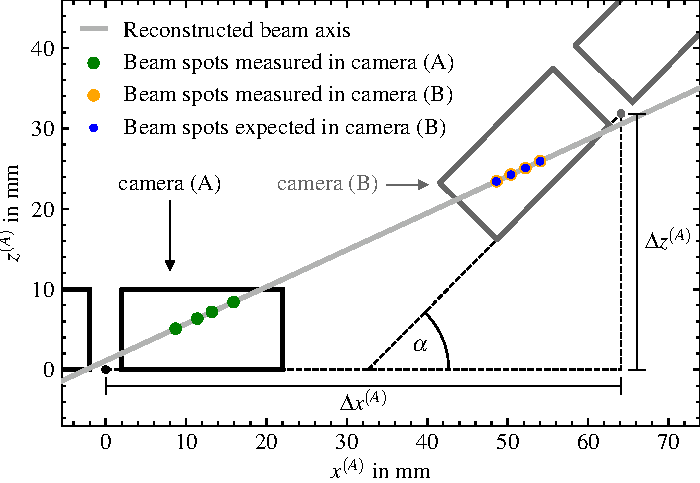
\includegraphics{figs/scanner/Camera_alignment_A.pdf}
	\caption{A depiction of the camera A-B alignment described in the text. The horizontal motor track is represented as a thick gray line intersecting both cameras. The expected beam spots in blue are derived from the motor coordinates, whereas the measured orange beam spots on camera (B) have been converted into the coordinate system of camera (A) with the coordinate transformation of Eq.~\ref{eq:czt_relative3D}. The ($x,z$)-origin of the local camera coordinate systems are shown as black (camera A) and gray (camera B) dots centered between the rectangles representing the CZT crystals~\cite{felix_comm}.}
	\label{fig:czt_relative2D}
\end{figure} 

The orientation of $y$ and the offset in this dimension, $\Delta y^{(A)}$, was determined by irradiating both cameras simultaneously from the side with the \CsS{} source unmounted~\cite{alignment_jan}.

Including this final rotation and offset, the coordinate transformation that takes the local camera (B) coordinates into the camera (A) coordinate system is as follows, 
\begin{equation}
     \left[\begin{array}{c} x^{(A)} \\ y^{(A)} \\ z^{(A)} \end{array}\right] = \underbrace{\left[\begin{array}{ccc} \cos(\alpha) &0 & \sin(\alpha) \\ 0 & 1 & 0 \\ -\sin(\alpha) & 0 & \cos(\alpha) \end{array}\right]}_\text{rotate by $\alpha$ around $y^{(B)}$} \underbrace{\left[\begin{array}{ccc} -1 & 0 & 0\\ 0 & -1 & 0 \\0 & 0 & 1 \end{array}\right]}_{\text{flip $x^{(B)}$ and $y^{(B)}$}} \left[\begin{array}{c} x^{(B)} \\ y^{(B)} \\ z^{(B)} \end{array}\right] \underbrace{+ \left[\begin{array}{c} \Delta x^{(A)} \\ \Delta y^{(A)} \\\Delta z^{(A)} \end{array} \right]}_{\makebox(0,0){$\scriptstyle \text{translate center (B) to (A)}$}}~, \label{eq:czt_relative3D}
\end{equation}
with $\alpha = 45.37^\circ$, $\Delta x^{(A)} = (64.13\pm0.03)\,\text{mm}$, $\Delta y^{(A)} = (0.45\pm0.03)\,\text{mm}$ and $\Delta z^{(A)} = (31.86\pm0.02)\,\text{mm}$ (statistical uncertainties)~\cite{felix_comm}.

\subsection{Motor Control} \label{subsec:motorcontrol}
The translational and rotational motor stages are driven via the motor control system. At the heart of this system, a triple axis stepper motor controller (Trinamic\textsuperscript{\tiny\textregistered} TMCM-3110~\cite{trinamic}) provides power and is able to drive all three motor stages simultaneously, introducing minimal vibrations. However, oscillations have been observed in detector signals during motor operation. For this reason, motors are never operated during data acquisition, and no data is taken in the 1\,s interval after motor operation. 
\begin{figure}[htb]
	\centering
	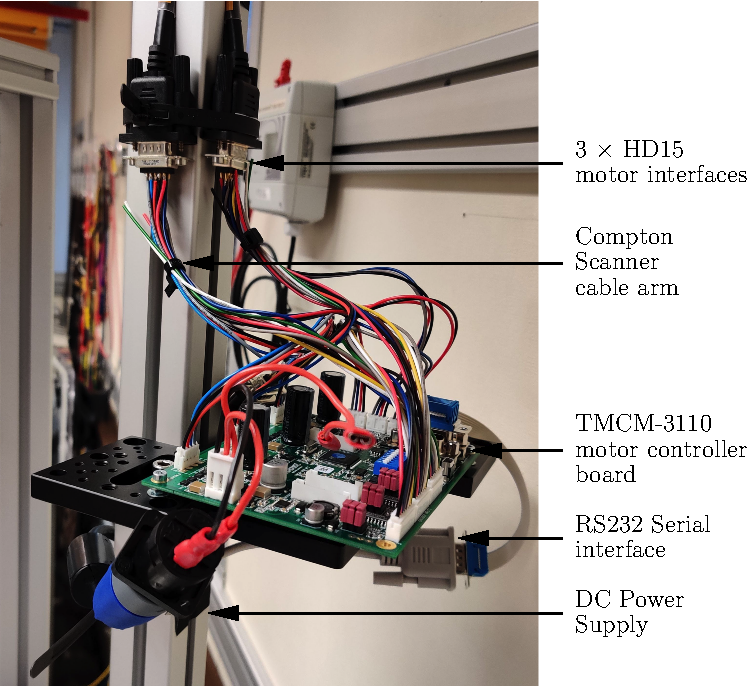
\includegraphics[width=5in]{figs/scanner/motor_control_labeled_width_5in.png}
	\caption{The fully operational motor control system prior to enclosure installation.}
	\label{fig:motorcontroller}
\end{figure}
The motor control system was built and programmed to interface with the two translational and one rotational motor stages (each controlled by a separate channel on the TMCM-3110 board). Thus, the system is fully customizable, allowing the user to set such motor parameters as acceleration, speed, and switch operation, on a channel by channel basis. These parameters were chosen with the load on each motor in mind to carefully and smoothly drive each motor stage. 
%A correctly programmed hardware switch will switch off a motor if it reaches the end of its track. However, this does not stop the motor if it encounters other objects in its path. This poses a problem for the vertical and horizontal motor stages, whose tracks could cause a collision between the source and camera. To remedy this a software switch was introduced which impedes the user from moving the camera into the path of the source. 

The user interfaces with the motor control system with a \julia{} software package. The package was designed to send encoded commands to the TMCM-3110's serial interface via a NetCom Plus 811 serial server. With this software the user can type simple command line instructions - such as move, calibrate, stop - via any terminal running \julia{} allowing for remote control of all motors via ssh. A network camera mounted on the crossarm aids in the safe remote operation of the motor system. 

\section{Commissioning Data}

An n-type segmented point-contact germanium detector with an energy resolution of 2.63\,keV at 356\,keV was used to take Compton scanner commissioning data. Monte Carlo simulations indicate that this energy resolution, and the geometry of the system, result in ``a FWHM resolution of less than $\pm1\,\text{mm}$ along the beam direction''~\cite{compton_scanner}. This detector was chosen because of the wealth of information the segmentation provides. Each event results in four pulses, corresponding to the point-contact and the three-fold segmentation contact readout. Thus, a single reconstructed event provides four pulses which can be compared to simulation. A pulse shape library was created for this detector along the $\langle100\rangle$ crystallographic axis and compared to \SSD{} simulations. The trends observed in data and simulation agree, which cross validated the position reconstruction described in this chapter and the fidelity of \SSD{} simulations for this detector. The commissioning data demonstrated that the goals of the Compton scanner -- most succinctly the $\pm1\,\text{mm}$ FWHM position reconstruction resolution and the drastic reduction in scanning times -- were met, paving the way for the application of the system to the next generation of Ge detectors. 